\documentclass[11pt, oneside]{article}   	% use "amsart" instead of "article" for AMSLaTeX format
\usepackage{geometry}                		% See geometry.pdf to learn the layout options. There are lots.
\geometry{letterpaper}                   		% ... or a4paper or a5paper or ... 
%\geometry{landscape}                		% Activate for rotated page geometry
%\usepackage[parfill]{parskip}    		% Activate to begin paragraphs with an empty line rather than an indent
\usepackage{graphicx}				% Use pdf, png, jpg, or eps§ with pdflatex; use eps in DVI mode
								% TeX will automatically convert eps --> pdf in pdflatex		
\usepackage{amssymb}
\usepackage{gensymb}

%SetFonts

%SetFonts


\title{An integrated fission gas swelling correlation for UMo research reactor fuel}
\author{Benjamin Beeler, Bei Ye, Jahid Hasan, Zhi-Gang Mei, Hakan Ozaltun}
\date{}							% Activate to display a given date or no date

\begin{document}
\maketitle
%\section{}
%\subsection{}

Equations are built with nominal parameters as the basis. Thus, comparing this set of equations to the INL swelling correlation requires the nominal parameters. Nominal grain size is 8.5 $\mu$m, nominal fission rate density is 5.94$\times$10$^{14}$ fiss/cm$^3$-s. Currently, data is fit to a range from 4.4 $\mu$m to 17 $\mu$m, and 3$\times$10$^{14}$ fiss/cm$^3$-s to 9$\times$10$^{14}$ fiss/cm$^3$-s. However, the expected range of applicability is anticipated to be beyond these ranges. 

\begin{equation}
\label{eq:FGS}
FGS\% = [f_1(f_d,D)\times f_c(f_d) + f_2(f_d,D)]\times f_3(\dot{f})
\end{equation}

\begin{equation}
\label{eq:f1}
f_1 = \frac{a\times D^b}{1+ exp(-(c\times D^d)\times (f_d - (e\times D^f))}
\end{equation}

\begin{equation}
\label{eq:fc}
f_c = \frac{1}{1+ exp(-50\times (f_d - 0.2 ))}
\end{equation}

\begin{equation}
\label{eq:f2}
f_2 = \frac{g\times ln(D) + h}{1+ exp(-(j\times D^k)\times (f_d - (l\times D^m))}
\end{equation}

\begin{equation}
\label{eq:fdot}
f_3 = 7.3449 \times 10^{-31} \times \dot{f}^2 + 3.5975 \times 10^{-16} \times \dot{f} + 0.52716
\end{equation}

\begin{table}[htp]
\caption{Parameters to equations \ref{eq:f1} and \ref{eq:f2}.}
\begin{center}
\begin{tabular}{|c|c|}
\hline
Coefficient & Value \\
\hline
a	&	14.38441	\\
b	&	0.82458	\\
c	&	2.6274	\\
d	&	-1.17587	\\
e	&	0.97384	\\
f	&	1.54856	\\
g	&	3.12897	\\
h	&	-0.44803	\\
j	&	3.16271	\\
k	&	0.27553	\\
l	&	16.26997	\\
m	&	15.99187	\\
\hline
\end{tabular}
\end{center}
\label{default}
\end{table}%


We can implement temperature as well once standard are implemented for cross-code validation of inlet/centerline temperature. This is for a reference of starting centerline temperature. Alternately stated as beginning of life, full power, centerline temperature. The nominal value is 150 \degree C.

\begin{equation}
f_4(T) = 0.0088 \times T - 0.3235
\end{equation}

An example of the fission gas swelling as a function of fission density for three different grain sizes is shown in Fig. \ref{fig:1}, where the grain sizes are shown in the legend and provided in units of $\mu$m. The 8.5 $\mu$m case is considered the nominal case. As can be seen, a smaller grain size leads to more rapid swelling and a larger total swelling at the end of life. Conversely, larger grain size leads to a more gradual swelling behavior. 

\begin{figure}[htbp]
\begin{center}
\label{fig:1}
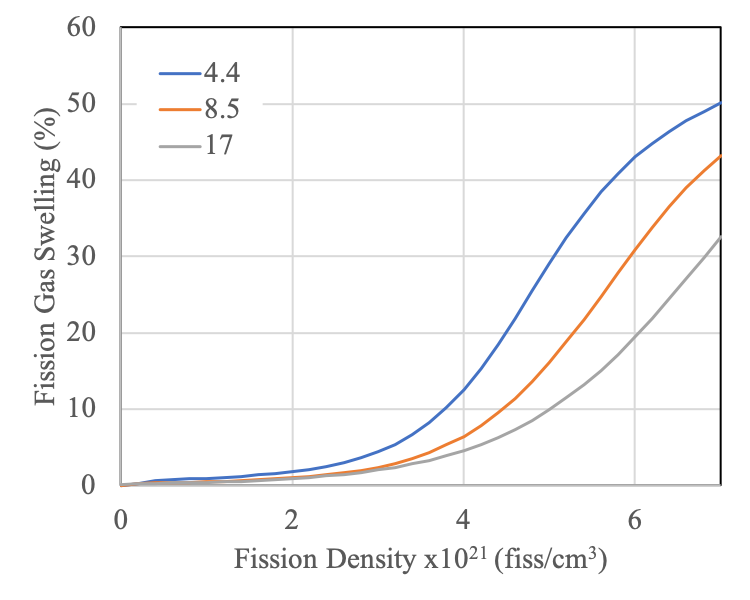
\includegraphics[width=0.75\textwidth]{Picture1.png}
\caption{Fission gas swelling as a function of fission density at three unique grain sizes.}
\label{default}
\end{center}
\end{figure}

An example of the effect of fission rate density is shown in Fig. \ref{fig:2}, where the fission gas swelling as a function of fission density at three fission rates densities is shown. An increase in the fission rate density, at the same fission density, tends to increase the amount of swelling. The data shown is for the 4.4 $\mu$m grain size. Currently, the fission rate density dependence does not have a grain size dependence. 

\begin{figure}[htbp]
\begin{center}
\label{fig:2}
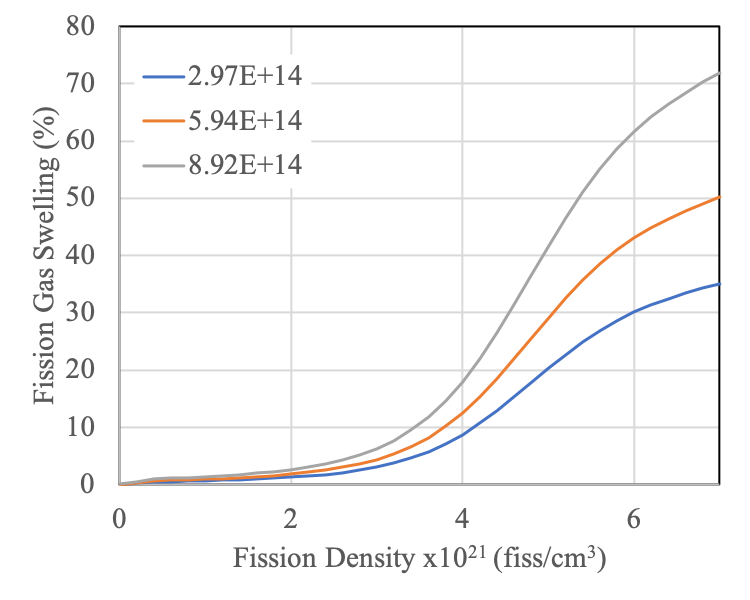
\includegraphics[width=0.75\textwidth]{Picture2.png}
\caption{Fission gas swelling as a function of fission density at three unique fission rate densities.}
\label{default}
\end{center}
\end{figure}




\end{document}  